\chapter{Our approach}
In authorship attribution problems, there is a set of candidate authors and a set of
text samples in the training set covering some of the works of the authors. In the
test dataset, there are samples of texts and each of them needs to be attributed to
a candidate author.
In the next sections, we are going to describe the experiment we carried out taking care of the chronological path of the events.
Our main focus has always been on closed set authorship attribution, training with instance-based approach (i.e. extracting features by not considering the other available text samples in the training).
The three milestones can be summarized as follows:
\begin{enumerate}
	\item Dataset selection and preparation
	\item Method selection
	\item Features extraction
\end{enumerate}

\section{Dataset preparation}
In section 4.6 we have already shown the datasets we selected. In particular, in this section we are going to show the procedures done to prepare the datasets for the next steps. For the single topic authorship attribution task we decided to select the RCV1 dataset, the dataset of 45 Victorian era book authors from the GDELT project and the dataset of amazon food reviews collected in the first decade of the 2000s. Regarding the cross domain authorship attribution task, we selected the dataset extracted from The Guardian newspaper.

\subsection{Reuters Corpus}
It consists of a collection of newswire stories written in English that cover four main topics: corporate/industrial (CCAT), economics (ECAT), government/social (GCAT) and markets (MCAT).
We sent a request to obtain the dataset on this webpage \url{https://trec.nist.gov/data/reuters/reuters.html}.
After few days, we gathered the RCV1 Corpus as it contains 810,000 Reuters, English Language News stories (about 2.5 GB).
First of all we had to convert the dataset, that contained folders of xml files, into a big csv with author's labels and document text.
\autoref{lst:RCV1Extraction} shows the process of documents and authors extraction, using `xml` python library. We decided to take into account this properties of the document: \textit{text, title, headline, byline, dateline, lang, corpus\_path, corpus\_subdirectory, corpus\_filename}.


\begin{lstlisting}[frame=none,caption={Extract and Parse RCV1 XML document into csv.},captionpos=b,label=lst:RCV1Extraction]
\end{lstlisting}
\begin{python}	
	import os
	import xml.etree.ElementTree as ET

	for f in files:
		try:
			data_path = os.sep.join([dir_path, f])
			raw_data = open(data_path).read()
			try:
				xml_parse = ET.fromstring(raw_data)
			except:
				print(D,"/",f,"failed to parse XML.")
				continue
		
			def get_text(tag): 
				stuff = xml_parse.find(tag)
				if stuff: 
					return stuff.text
				else: 
					return None
	
		text = "\n\n".join([str(p.text) for p in xml_parse.findall(".//p")])
		title = get_text("title")
		headline = get_text("headline")
		byline = get_text("byline")
		dateline = get_text("dateline")
		
		#this bit got funky in the XML parse
		lang_key = [k for k in xml_parse.attrib if "lang" in k][0]
		lang = xml_parse.attrib[lang_key]
	
		code_classes = [c.attrib["class"] 
		for c in xml_parse.findall(".//codes")]
		codes = {cc: [c.attrib["code"] for c in 
			xml_parse.findall(".//codes[@class='%s']/code"%cc)]
			for cc in code_classes}
		dcs = {d.attrib["element"]: d.attrib["value"] 
			for d in xml_parse.findall(".//dc")}
		
		#assemble output
		output = {"text": text,
			"title": title,
			"headline": headline,
			"byline": byline,
			"dateline": dateline,
			"lang": lang,
			"corpus_path": corpus_path,
			"corpus_subdirectory": D,
			"corpus_filename": f,
		}
		
		# merge and flatten the other big hashmaps
		output.update(codes.items())
		output.update(dcs.items())
		
		result.append(output)
	except Exception as e:
		print(e)
\end{python}

The dataset was then filtered only with the documents with a \textit{\enquote{byline}} property defined. We end up with 109'433 documents written by 2400 distinct authors. At this point, we labeled this portion of the RCV1 original dataset as the \textit{\enquote{Full RCV1 dataset}}.
In order to test and compare our approach, reproducing the testing scenario
described in previous research \cite{stamatatos2009survey}, the 10 most prolific authors were chosen from the CCAT category, and then, 50 examples per author for training and 50 examples for testing were selected randomly with no overlapping between training and testing sets. We will reference to this portion of the RCV1 dataset as the \textit{\enquote{RCV1\_10}}.
In previous works \cite{houvardas2006n}, the authors proposed another adaptation of the RCV1 corpus for the authorship attribution task. They choose the 50 most prolific authors from the Reuters Corpus, keeping 50 examples per author for training and 50 examples per author for testing with no
overlapping between them. We will refer to this corpus as the \textit{RCV1\_50}.\\
The RCV1\_10 and RCV1\_50 datasets are both balanced over different authors and have their genre fixed to news.
The majority of our work has been conducted on the RCV1\_50, although to compare results with previous works we will show also the same techniques applied to the RCV1\_10 corpus.
\autoref{tab:tableRCV1kpi} shows the main metrics to describe these different portions of the original dataset.

\begin{table}[h!]
	\begin{center}  
		\caption[Reuters Corpus metrics]{Main metrics to describe different portion of the Reuters Corpus dataset.} 
		\label{tab:tableRCV1kpi}
		%\resizebox{\linewidth}{!}{  %
		\begin{tabular}{|c | c | c | c | c |}
			\hline 
			Name & N\# docs & N\# authors & Avg docs length & Avg n\# docs/author \\
			\hline
			Full RCV1 & 109433 & 2400 & 3061.95 & 45.60 \\ \hline
			RCV1\_10 & 1000 & 10 & 3093.82 & 100  \\ \hline
			RCV1\_50 & 5000 & 50 & 3251.16 & 100  \\ \hline
			%\bottomrule 
		\end{tabular} 
		%}
	\end{center}
\end{table}

\subsection{GDELT}
The GDELT Project is one of the largest publicly available digitized book database which has more than 3.5 million books published from 1800-2015. The GDELT Project is an open platform for research and analysis of global society and thus all datasets released by the GDELT Project are available for unlimited and unrestricted use for any academic, commercial, or governmental use of any kind without any fee\footnote{\url{https://www.gdeltproject.org/about.html}}. The whole digitized dataset is publicly available and interested researchers can freely perform SQL queries using the Google big query platform. For example; the book names, publication year, quotations, themes, the original text of the book of “Mark Twain” which were written between 1890 to 1900 can be found as follows
using the Big query platform of Google in \autoref{lst:bigQuerySQL}.
\begin{lstlisting}[linewidth=18cm, frame=none,caption={Google Big Query on GDELT.},captionpos=b,label=lst:bigQuerySQL]
\end{lstlisting}
\begin{lstlisting}
SELECT Themes, V2Themes, Quotations, AllNames, 
TranslationInfo, BookMeta_Identifier, BookMeta_Title, 
BookMeta_Creator, BookMeta_Subjects, BookMeta_Year,
FROM (TABLE_QUERY([gdelt-bq:internetarchivebooks],
'REGEXP_EXTRACT(table_id, r"(\d{4})") BETWEEN "1890" 
AND "1900"'))
WHERE BookMeta_Creator CONTAINS "Mark Twain"
LIMIT 50
\end{lstlisting}

To decrease the bias and create a reliable dataset the following criteria have been chosen to filter out authors: English language writing authors, authors that have enough books available (at least 5), 19th century authors. With these criteria 50
authors have been selected and their books were queried through Big Query Gdelt
database. The next task has been cleaning the dataset due to OCR reading problems
in the original raw form. To achieve that, firstly all books have been scanned through
to get the overall number of unique words and each words frequencies. While scanning
the texts, the first 500 words and the last 500 words have been removed to take out
specific features such as the name of the author, the name of the book and other word
specific features that could make the classification task easier. After this step, we have
chosen top 10, 000 words that occurred in the whole 50 authors text data corpus. The
words that are not in top 10, 000 words were removed while keeping the rest of the
sentence structure intact. Afterwards, the words are represented with numbers from
1 to 10, 000 reverse ordered according to their frequencies. The entire book is split
into text fragments with 1000 words each. We separately maintained author and
book identification number for each one of them in different arrays. Text segments
with less than 1000 words were filled with zeros to keep them in the dataset as well.
1000 words make approximately 2 pages of writing, which is long enough to extract a variety of features from the document. The reason why we have represented top
10, 000 words with numbers is to keep the anonymity of texts and allow researchers
to run feature extraction techniques faster. Dealing with large amounts of text data
can be more challenging than numerical data for some feature extraction techniques.
When gathering the dataset, we decided to discard 5 authors for which their writings were not consistent enough for the authorship attribution task.
We ended up with a full dataset with 53'678 documents instances, each one containing 1000 words.
In order to make training methods reliable across dataset, we decided to select 100 documents of each authors, with a 50/50 split (i.e. 50 documents in the training set, 50 documents in the testing set, no overlapping among them). In the following sections, we will refer to this as the \textit{"GDELT\_45"}.
\autoref{tab:tableGDELTkpi} shows the metrics that describe best this dataset.

\begin{table}[h!]
	\begin{center}  
		\caption[GDELT Corpus metrics]{Main metrics to describe different portion of the GDELT Corpus dataset.} 
		\label{tab:tableGDELTkpi}
		%\resizebox{\linewidth}{!}{  %
		\begin{tabular}{|c | c | c | c | c |}
			\hline 
			Name & N\# docs & N\# authors & Avg docs length & Avg n\# docs/author \\
			\hline
			Full GDELT & 53678 & 45 & 4950.61 & 1192.84 \\ \hline
			GDELT\_45 & 4500 & 45 & 4911.91 & 100  \\ \hline
			%\bottomrule 
		\end{tabular} 
		%}
	\end{center}
\end{table}

\subsection{Amazon Food Reviews}
This dataset consists of reviews of fine foods from amazon. The data span of over a period of more than 10 years, including all ~500,000 reviews up to October 2012. Reviews include product and user information, ratings, and a plain text review. It also includes reviews from all other Amazon categories.
We decided to consider this dataset for our experiment, because we were missing a more \enquote{everyday} example of dataset to work with. As \autoref{tab:tableAFRkpi} shows, the average documents length is dramatically lower than the other two datasets presented previously, providing us with a good challenge to show consistency of our method across all these different scenarios.
Moreover, in order to make training methods reliable across dataset, we decided to select 100 reviews of each customers, with a 50/50 split (i.e. 50 reviews in the training set, 50 reviews in the testing set, no overlapping among them). In the following sections, we will refer to this as the \textit{"AFR\_50"}.

\begin{table}[h!]
	\begin{center}  
		\caption[Amazon Food Reviews Corpus metrics]{Main metrics to describe different portion of the Amazon Food Reviews dataset.} 
		\label{tab:tableAFRkpi}
		%\resizebox{\linewidth}{!}{  %
		\begin{tabular}{|c | c | c | c | c |}
			\hline 
			Name & N\# docs & N\# authors & Avg docs length & Avg n\# docs/author \\
			\hline
			Full AFR & 568454 & 256059 & 380.70 & 2.2 \\ \hline
			AFR\_50 & 5000 & 50 & 990.45 & 100  \\ \hline
			%\bottomrule 
		\end{tabular} 
		%}
	\end{center}
\end{table}

\subsection{The Guardian newspaper}
\label{ssec:guardian}
Although the majority of our time and effort was focused on the first 3 single domain datasets for closed set authorship attribution task, we wanted to test our approach with a cross domain dataset.
\textit{The Guardian corpus} is composed of texts published in The Guardian daily newspaper. The majority of the corpus comprises opinion articles
(comments). The newspaper describes the opinion articles using a set of tags indicating its subject. There are eight top-level tags (World, U.S., U.K., Belief, Culture, Life\&Style, Politics, Society), each one of them having multiple subtags.
In order to test and compare our approach, we reproduce the testing scenario
described in the previous research \cite{stamatatos2013robustness} using the Guardian corpus. The experimental
scenario is as follows: 
\begin{enumerate}
	\item Select at most ten samples per author in each topic category
	(in \autoref{fig:tgc_dataset} we can see the distribution of the samples per author for the Politics category after considering
	the restriction of ten samples per author)
	\item Use the samples in the Politics category as training set and train the classifier
	\item Finally, test the classifier using
	another topic category different from Politics (four possible pairings)
\end{enumerate}

\begin{figure}[ht]
	\centering
	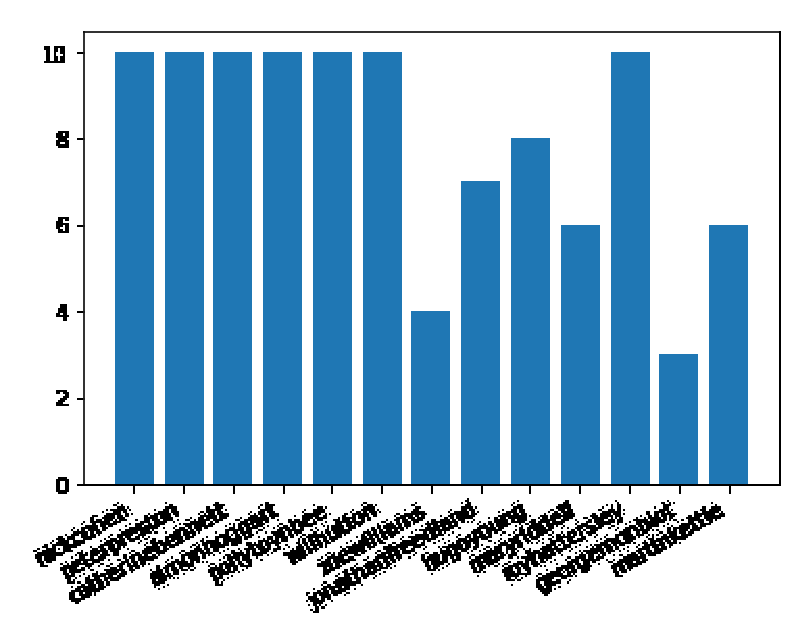
\includegraphics[width=1.0\textwidth, height=1.0\textheight, keepaspectratio]{theguardian_dataset}
	\caption[The Guardian Politics samples distribution]{The Guardian samples distribution for the Politics topic.}
	\label{fig:tgc_dataset}
\end{figure}

\section{Features extraction}
After the choice of dataset and classification method, all our energies were spent on the choice of feature extraction. In order to identify the authorship of an unknown text document using machine learning the document needs to be quantified first. The simple and natural way to characterize a document is to consider it as a sequence of tokens grouped into sentences where each token can be one of the three: word, number, punctuation mark.
As with the choice of classification method, we initially attempted a naive approach. In fact, many studies have focused on using methods such as TFIDF and Bag Of Words. In fact, our experiment is mainly aimed at showing that simple numerical text representation methods such as TFIDF or BOW, applied with the right hyperparameters, can somehow yield good performance in the same way as other more complex methods such as Doc2Vec or n-grams character selection.
\subsection{Term Frequency - Inverse Document Frequency \& Bag Of Words}
Once taken the route of the simple feature extraction approach via TFIDF and BOW, we had to choose the hyperparameters that would play a main role in the model performances for this task. 
We initially chose a classical approach to the problem, extracting features with both TFIDFVectorizer and CountVectorizer, with standard hyperparameters.


In \autoref{lst:vectorizers} we can see the initialization of the vectorizers with the chosen hyperparameters after a long process of tuning and validation.

\begin{lstlisting}[frame=none,caption={TFIDF \& BOW Vectorizer.},captionpos=b,label=lst:vectorizers]
\end{lstlisting}
\begin{python}	
	tfidf_vec = TfidfVectorizer(max_df=0.75, max_features=None,
	min_df=0.02, use_idf=False, tokenizer=custom_tokenizer, 
	ngram_range=(1, 4))
	counter_vect = CountVectorizer(max_df=0.8, max_features=10000,
	min_df=0.02, tokenizer=custom_tokenizer, ngram_range=(1, 2))
\end{python}

After that, we shifted our focus to the tokenizer that instead of choosing to use the standard one, we preferred to use a \enquote{custom} one. We initially used a robust tokenizer for text categorization tasks, but we realized that for this kind of authorship attribution problem, some approaches valid for many text categorization problems would not work.
In fact, in \autoref{lst:tokenizers} shows the choice of the three tokenizers we tried experimentally and which sequentially showed better and better results. The first one we tried was a custom tokenizer with classical approaches to text categorization. In fact, we used a \enquote{snowball} type stemmer for the English language and applied it to all the filtered words. We also converted all words to lowercase and removed the words from the English stopwords group. This type of tokenizer proved to be the weakest of the three because it removes too many features that best distinguish and characterize a text with respect to the author of the document itself.

\begin{lstlisting}[frame=none,caption={Custom tokenizer for TFIDF and BOW.},captionpos=b,label=lst:tokenizers]
\end{lstlisting}
\begin{python}	
	def tokenize_and_stem(text):
		"""
		Below function tokenizes and lemmatizes the texts. It also does some cleaning by removing non dictionary words
		This can be used to replace default tokenizer provided by feature extraction api of sklearn.
		:param text: str
		:return: list
		"""
		stemmer = SnowballStemmer("english")
		stop_words = stopwords.words("english")
		tokens = [word.lower() for sent in nltk.sent_tokenize(text) for word in nltk.word_tokenize(sent)]
		filtered_tokens = []
		for token in tokens:
			if re.search(r'[a-zA-Z-]{4,}', token) and token not in stop_words and len(wn.synsets(token)) > 0:
				token.strip()
				filtered_tokens.append(token)
		filtered_tokens = [stemmer.stem(token) for token in filtered_tokens]
	return filtered_tokens
	
	def simple_tokenizer(text):
		text = re.sub('"([^"]*)"', '', text)
		tokens = [word.lower() for sent in nltk.sent_tokenize(text) for word in nltk.word_tokenize(sent)]
		filtered_tokens = []
		for token in tokens:
			if len(wn.synsets(token)) > 0:
				token.strip()
				filtered_tokens.append(token)
		return filtered_tokens
	
	def only_remove_quoting_tokenizer(text):
		text = re.sub('"([^"]*)"', '', text)
		tokens = [word.lower() for sent in nltk.sent_tokenize(text) for word in nltk.word_tokenize(sent)]
		return tokens
\end{python}


In fact, the approach of purposely modifying words and removing stopwords, in the literature on authorship attribution has proven to be a wrong one. The most frequent words defined as \enquote{non-content} categorize worse a text in the sense of content and introduce noise, but better classify a text in respect of the author who wrote it, especially in cross domain contexts in which are precisely the content words that go to introduce noise.
After evaluating our results with the available datasets, we agreed to change our approach regarding the tokenizer. We tried to build a simpler tokenizer called \textit{\enquote{simple\_tokenizer}} that would remove only the words between double-quotes because they were considered as phrases or quotation words and therefore would not classify well the text in respect of the author who reported them, after which we only removed those words that, after transforming them into lowercase, were not found as synonyms of an English dictionary (and therefore words that do not conform to the dictionary). This second approach showed better results than the first, but once again we wondered if the approach of removing words that did not conform to the dictionary was a correct approach for author attribution analysis. With these premises in fact, in the third and last approach we thought to remove only the words or phrases contained in quotation marks, without removing the words therefore wrong or not present in the official dictionary of the English language. This last approach, called \textit{\enquote{only\_remove\_quoting\_tokenizer}} proved to be the best of the three, thus underlining the importance of stopwords and common mistakes or words commonly used by the author and not present in the official English dictionary, regarding this specific task of authorship attribution.
Just for the purpose of making the reader aware, as a tokenizer we tried two additional approaches but they did not show the desired results.  Along the lines of thinking that the content words of a text are the ones that litter the numerical representation of a text the most in an authorship attribution context, one of the approaches attempted was text distortion. In fact as also shown in some previous articles \cite{stamatatos2017authorship}, using text distortion for autorship attribution tasks, especially in cross domain contexts, could be very effective. The concept behind text distortion is to obfuscate and hide words in a document based on their frequency, so as not to create noise during feature extraction and focus only on the most relevant words. In the case of authorship attribution, the opposite is applied, i.e. less frequent words in a text are obfuscated (i.e. replaced by symbols like $ * $ and $ \# $) and the same applies to numbers. This approach can be divided into two: an approach that is length-preserving and an approach that particularly shortens the length of the text in order to make feature extraction even easier. In the first case we replace all letters of the selected target word with $ * $ or $ \# $ symbols for numbers, in the second case we replace the selected word with only one $ * $ or $ \# $ symbol for numbers, shortening the resulting text.
We applied both of these two approaches as tokenizers of TFIDF and BOW, but the results obtained did not even pass the threshold of mention as they were considered completely unsuccessful.

\subsection{Grid Search Cross Validation}
In almost any Machine Learning project, we train different models on the dataset and selecting the one with the best performance. However, there is almost a room for improvement as we cannot say for sure that this particular model is best for the problem at hand, hence our aim is to improve the model in any way possible. One important factor in the performances of these models are their hyperparameters, once we set appropriate values for these hyperparameters, the performance of a model can improve significantly. At the state of the art, we can say that one of the well-established approaches is to optimize the values of the hyperparameters of a model using GridSearchCV.
Note that there is no way to know in advance the best values for hyperparameters so ideally, we need to try all possible values to know the optimal values. Doing this manually could take a considerable amount of time and resources and thus we use GridSearchCV to automate the tuning of hyperparameters.
GridSearchCV is a function that comes in Scikit-learn’s model\_selection package. This function helps to loop through predefined hyperparameters and fit the model on the training set. So, in the end, we can select the best parameters from the listed hyperparameters.
As mentioned above, we pass predefined values for hyperparameters to the GridSearchCV function. We do this by defining a dictionary in which we mention a particular hyperparameter along with the values it can take.

\begin{lstlisting}[frame=none,caption={GridSearchCV with BOW, TFIDF and SGD.},captionpos=b,label=lst:gridsearchcv]
\end{lstlisting}
\begin{python}	
	pipeline = Pipeline([
	('vect', CountVectorizer()),
	('tfidf', TfidfTransformer()),
	('clf', SGDClassifier()),
	])
	
	# uncommenting more parameters will give better exploring power but will
	# increase processing time in a combinatorial way
	parameters = {
		'vect__max_df': (0.5, 0.75, 1.0),
		'vect__max_features': (None, 5000, 10000, 50000),
		'vect__ngram_range': ((1, 1), (1, 2)),  # unigrams or bigrams
		'tfidf__use_idf': (True, False),
		'tfidf__norm': ('l1', 'l2'),
		'clf__max_iter': (20,),
		'clf__alpha': (0.00001, 0.000001),
		'clf__penalty': ('l2', 'elasticnet'),
		'clf__max_iter': (10, 50, 80,),
	}
	
	# find the best parameters for both the feature extraction and the
	# classifier
	grid_search = GridSearchCV(pipeline, parameters, n_jobs=-1, verbose=1)
	
	print("Performing grid search...")
	print("pipeline:", [name for name, _ in pipeline.steps])
	print("parameters:")
	print(parameters)
	t0 = time.time()
	grid_search.fit(dataset['articles'], dataset['author'])
	print("done in %0.3fs" % (time.time() - t0))
	print()
	
	print("Best score: %0.3f" % grid_search.best_score_)
	print("Best parameters set:")
	best_parameters = grid_search.best_estimator_.get_params()
	for param_name in sorted(parameters.keys()):
	print("\t%s: %r" % (param_name, best_parameters[param_name]))
\end{python}

 In \autoref{lst:gridsearchcv} we can see an example of GridSearchCV applied to the datasets with a simple pipeline with: CountVectorizer, TfidfTransformer and SGDClassifier. The pool of parameters we chose were based on previous research on same datasets.
GridSearchCV tries all the combinations of the values passed in the dictionary and evaluates the model for each combination using the Cross-Validation method. Hence after using this function we get accuracy/loss for every combination of hyperparameters and we can choose the one with the best performance. The result of this first attempt at GridSearchCV was shown in \autoref{lst:vectorizers}, the picture of the final hyperparameter tuning we mentioned earlier in the section.

\subsection{Vector embeddings of documents}

Since we did not want to rely only on some classical feature extraction methods such as TFIDF and BOW mentioned above, recent studies have shown how the use of techniques such as the vector spacing model that transforms document instances into vectors can be successfully applied to tasks such as autorship attribution. To make the reader understand better, the broad idea is to transform each author's documents into vectors of fixed size. These vectors will be \enquote{similar} for documents of the same author, so on documents of unknown author we will look for the collection of documents whose representation in vector format is closest to the vector representation of the document of unknown author.
We used the Doc2vec \cite{le2014distributed} method available in the freely downloadable GENSIM module in order to implement our proposal. The implementation of the Doc2vec method requires the following three parameters:
\begin{enumerate}
	\item the number of features to be returned (length of the vector)
	\item the size of the window that captures the neighborhood
	\item the minimum frequency of words to be considered into the model
\end{enumerate}

The values of these parameters depend on the used corpus. In a previous work \cite{posadas2017application} it reported a representation of 300 features, a window size equal to 10
and minimum frequency of 5. In \autoref{lst:doc2vectrain} we can see the implementation of the tagging document algorithm and the computation of the 2 different models for document embedding: Distributed Memory Model and Distributed Bag Of Words Model.

\begin{lstlisting}[frame=none,caption={Doc2Vec for features extraction with gensim python library.},captionpos=b,label=lst:doc2vectrain]
\end{lstlisting}
\begin{python}	
	from gensim.models.doc2vec import TaggedDocument
	import gensim
	from tqdm import tqdm
	from gensim.models import Doc2Vec
	
	def tag_dataset(df):
		return df.apply(lambda r: TaggedDocument(words=only_remove_quoting_tokenizer(r['articles']), tags=[r.author]), axis=1)
	
	df_train_tagged = tag_dataset(df_train)
	df_test_tagged = tag_dataset(df_test)
	
	import multiprocessing
	
	cores = multiprocessing.cpu_count()
	model_dmm = Doc2Vec(dm=1, dm_mean=1, vector_size=300, window=10, negative=5, min_count=1, workers=cores, alpha=0.065, min_alpha=0.065)
	model_dmm.build_vocab([x for x in tqdm(df_train_tagged.values)])
	
	model_dbow = Doc2Vec(dm=0, vector_size=300, negative=5, hs=0, min_count=2, sample = 0, workers=cores)
	model_dbow.build_vocab([x for x in tqdm(df_train_tagged.values)])
	
	d2v_model = model_dmm
	
	from sklearn import utils
	
	# time
	def train_d2v_model(model, df):
		for epoch in range(30):
			model.train(utils.shuffle([x for x in tqdm(df.values)]), total_examples=len(df.values), epochs=1)
			model.alpha -= 0.002
			model.min_alpha = model_dmm.alpha
		model.save(os.path.join(base_dir, 'd2v_{}_model.vec'.format(PROJECT_NAME)))
\end{python}

After the evaluation of both models, we decided to keep only the Distributed Memory Model which resulted in better performance in terms of the score values of the testing set.

\section{Method selection}
At this point, we had to face the problem of deciding the classifier method that would solve best our authorship attribution task.
Although in previous studies over the past decades on authorship attribution SVM has been shown to be very convincing (\cite{diederich2003authorship}, \cite{koppel2005determining}, \cite{zheng2006framework}), we initially wanted to construct an experimental approach that would lead us to exclude the other classifiers for our task.
\subsection{Manual approach}
Our very first naive approach was to compare on different portions of the dataset (increasing number of authors) different classification methods to see which one performed best.
Initially, we considered the authorship attribution study for groups of authors consisting of 6 or 10 authors. In truth, as many previous studies show, an authorship attribution model must perform well especially in situations where the group of authors is composed of several dozen candidates.
The classifiers initially chosen were:
\begin{itemize}
	\item Naive Bayes
	\item Multinomial Naive Bayes
	\item Logistic Regression
	\item XGBoost
	\item XGBoost with Neural Networks
	\item Random Forest
\end{itemize}

\begin{figure}[ht]
	\centering
	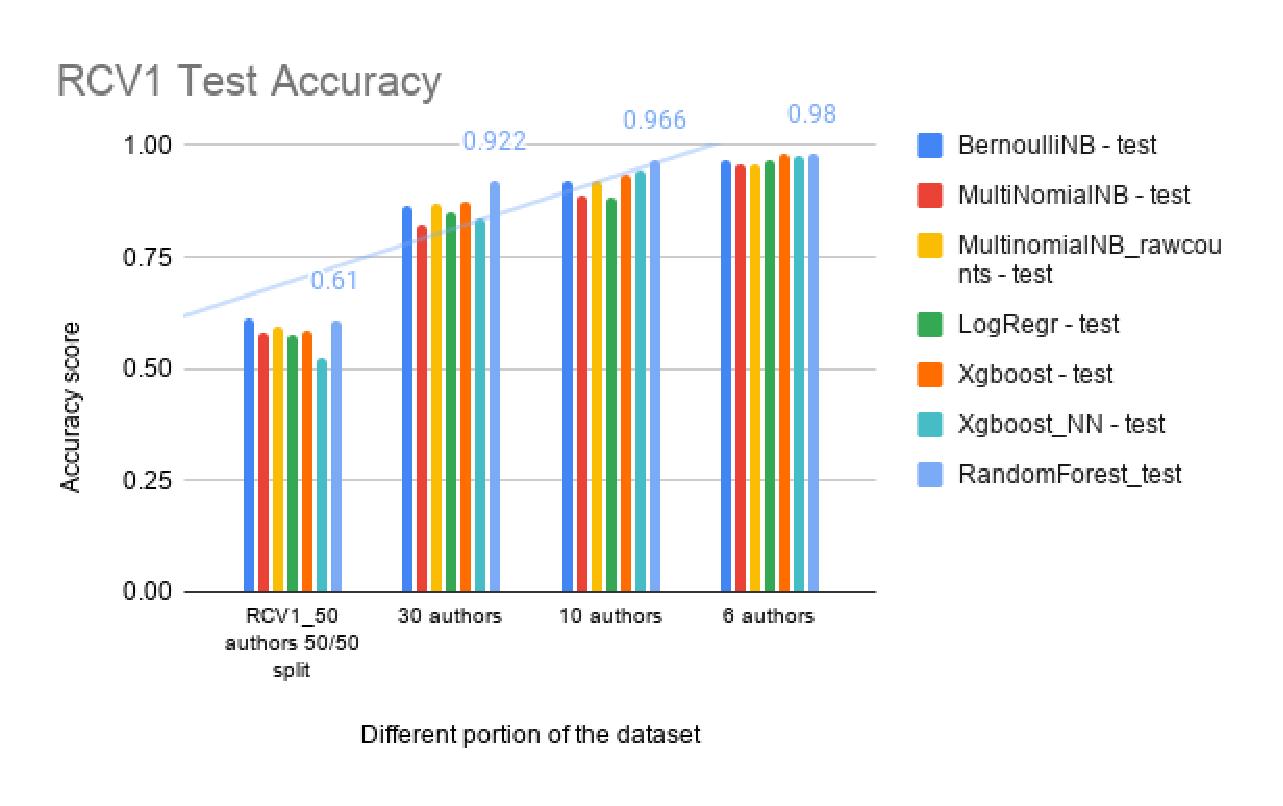
\includegraphics[width=1.0\textwidth, height=1.0\textheight, keepaspectratio]{RCV1_Test_Accuracy}
	\caption[Methods performance on Reuters Corpus]{Accuracy scores for different groups of authors on Reuters Corpus dataset.}
	\label{fig:RCV1_methods_accuracy}
\end{figure}

For text representation, we chose to use TFIDF and Bag Of Words, comparing the results depending on the dataset, the number of authors, and the method used.
In \autoref{fig:RCV1_methods_accuracy} we can see the accuracy score of the testing set of the various classifiers tested on the groups of authors increasing from right to left on the RCV1 dataset.

\begin{figure}[ht]
	\centering
	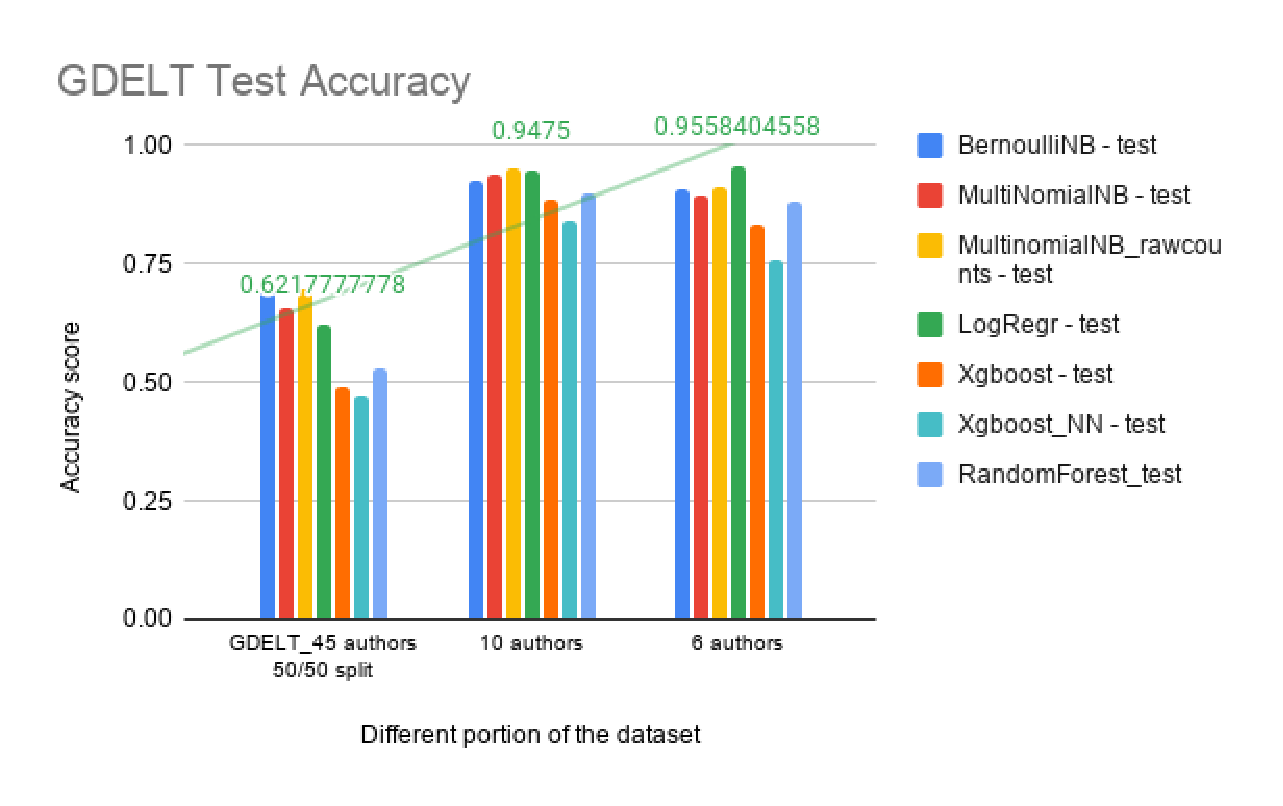
\includegraphics[width=1.0\textwidth, height=1.0\textheight, keepaspectratio]{GDELT_Test_Accuracy}
	\caption[Methods performance on GDELT corpus]{Accuracy scores for different groups of authors on GDELT corpus dataset.}
	\label{fig:GDELT_methods_accuracy}
\end{figure}

As on the groups of \enquote{small} authors, i.e. composed of 6 authors and 10 authors, almost all the classifiers exceed the threshold of 95\% accuracy that validates the approach even in non-research contexts. The classifier that seems to perform best among the various groups of authors increasing in number is RandomForest. On the other hand, it has been shown that decision tree type classifiers struggle to maintain high performance when the number of features used increases.

In fact in \autoref{fig:GDELT_methods_accuracy} and \autoref{fig:AFR_methods_accuracy} we can see that in all 3 single topic datasets the various methods proposed have a decrease in performance when the number of authors increases reaching 50 authors (or 45 in the case of the GDELT dataset).
This is probably due to the fact that by keeping the number of documents per author fixed at 50 in the training test (and in the testing set), the number of features to represent grows proportionately as the number of authors increases. Therefore, we need to select a classification method that remains stable as the number of features we want to represent increases, and therefore remains valid for 6, 10, 30, 50 authors (and more).


\begin{figure}[ht]
	\centering
	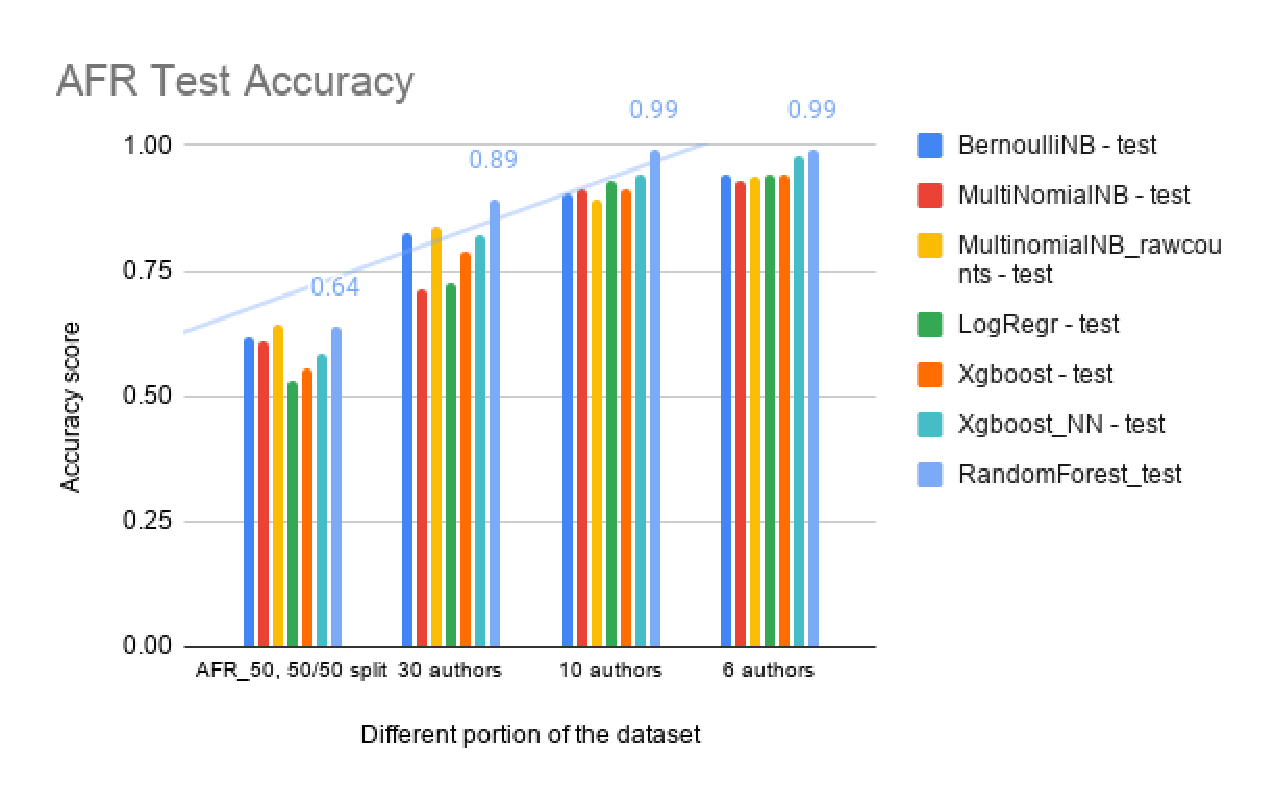
\includegraphics[width=1.0\textwidth, height=1.0\textheight, keepaspectratio]{AFR_Test_Accuracy}
	\caption[Methods performance on Amazon Food Reviews dataset]{Accuracy scores for different groups of authors on Amazon Food Reviews dataset.}
	\label{fig:AFR_methods_accuracy}
\end{figure}

\subsection{Tree-based Pipeline Optimization Tool}
Therefore, considering the more or less unsuccessful approaches of the methods presented in the previous section, we tried to find an approach that would validate our choice and those of previous works on the use of the Support Vector Machine as a classification method.
Our choice fell on Tree-based Pipeline Optimization Tool (TPOT)\footnote{\url{http://epistasislab.github.io/tpot/}}, an automated machine learning (autoML) tool in Python.
In order to give the reader of what TPOT is and how it works, we'll report the first paragraph quoting the TPOT website:

\begin{quote}
	TPOT is meant to be an assistant that gives you ideas on how to solve a particular machine learning problem by exploring pipeline configurations that you might have never considered, then leaves the fine-tuning to more constrained parameter tuning techniques such as grid search.
\end{quote}
So TPOT helps you find good algorithms. TPOT is built on the scikit learn library and follows the scikit learn API closely. It can be used for regression and classification tasks and has special implementations for medical research.
TPOT is open source, well documented, and under active development. It’s development was spearheaded by researchers at the University of Pennsylvania. TPOT appears to be one of the most popular autoML libraries, with more than 7,800 GitHub stars as of the moment of writing.
TPOT has what its developers call a genetic search algorithm to find the best parameters and model ensembles. It could also be thought of as a natural selection or evolutionary algorithm. TPOT tries a pipeline, evaluates its performance, and randomly changes parts of the pipeline in search of better performing algorithms (An example is shown in \autoref{fig:TPOT_pipeline}).
This power of TPOT comes from evaluating all kinds of possible pipelines automatically and efficiently. Doing this manually is cumbersome and slower.

\begin{figure}[ht]
	\centering
	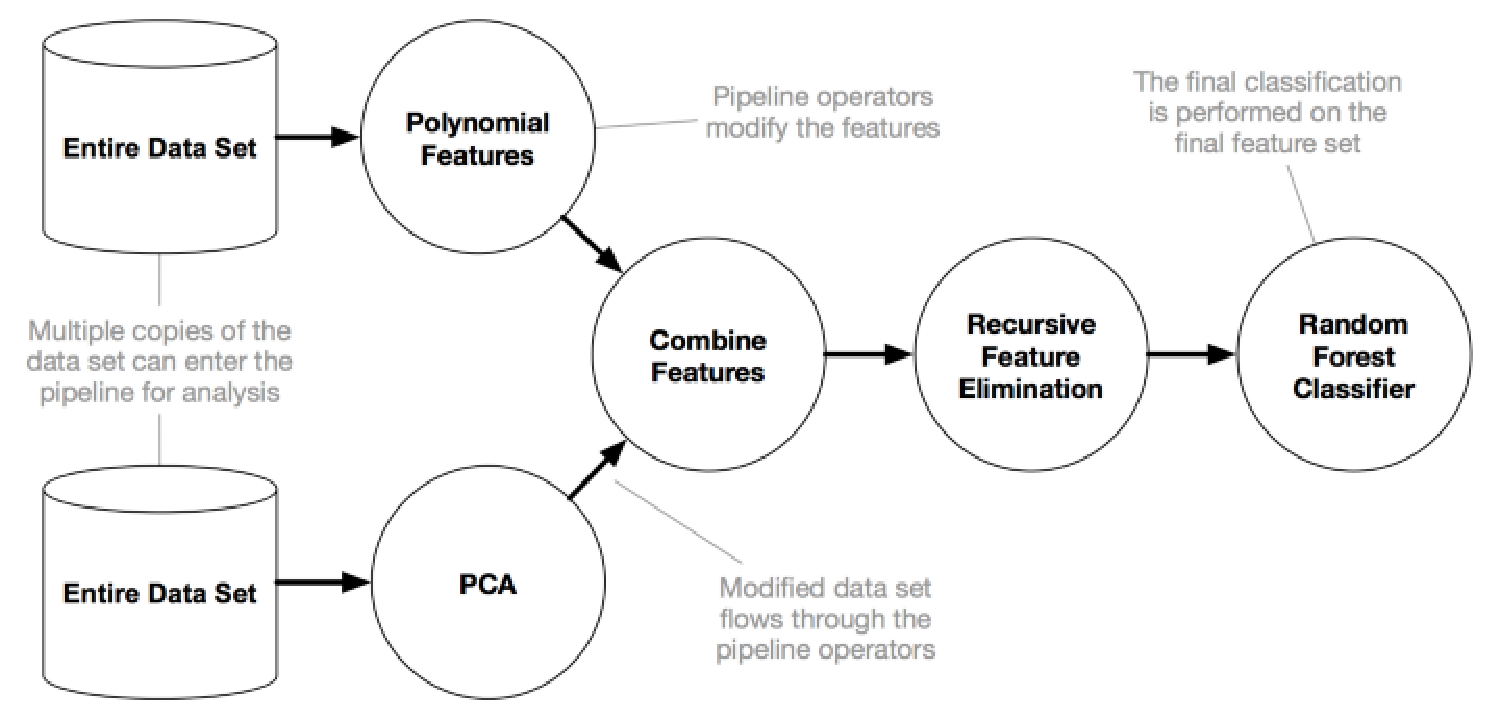
\includegraphics[width=1.0\textwidth, height=1.0\textheight, keepaspectratio]{TPOT_pipeline2}
	\caption[Tree-based Pipeline Optimization Tool pipeline example]{An example TPOT Pipeline from TPOT docs.}
	\label{fig:TPOT_pipeline}
\end{figure}

In \autoref{lst:TPOTpipeline} we show a snippet of code we used for extracting TPOT pipeline with hyper parameters and research space. 


\begin{lstlisting}[frame=none,caption={TPOT pipeline generation.},captionpos=b,label=lst:TPOTpipeline]
\end{lstlisting}
\begin{python}	
	!pip install -q tpot
	from tpot import TPOTClassifier, TPOTRegressor
	pipeline_optimizer = TPOTClassifier(generations=5, population_size=20, cv=5,
	random_state=42, verbosity=2, scoring='accuracy', config_dict='TPOT sparse')
	pipeline_optimizer.fit(tfidf_train, df_train['target'])
	print(pipeline_optimizer.score(tfidf_test, df_test['target']))
	pipeline_optimizer.export('tpot_exported_pipeline.py')
\end{python}

We chose the most appropriate hyperparameters and ran TPOT optimization pipelines on all 3 datasets with 50 authors \footnote{45 in the case of GDELT}. The result is shown in \autoref{lst:TPOTexported} for all 3 single domain selected datasets, thus proving that SVM is the best choice as a model classifier for this task.

\begin{lstlisting}[frame=none,caption={TPOT pipeline extracted.},captionpos=b,label=lst:TPOTexported]
\end{lstlisting}
\begin{python}	
	import numpy as np
	import pandas as pd
	from sklearn.model_selection import train_test_split
	from sklearn.svm import LinearSVC
	
	# NOTE: Make sure that the outcome column is labeled 'target' in the data file
	tpot_data = pd.read_csv('PATH/TO/DATA/FILE', sep='COLUMN_SEPARATOR', dtype=np.float64)
	features = tpot_data.drop('target', axis=1)
	training_features, testing_features, training_target, testing_target = \
	train_test_split(features, tpot_data['target'], random_state=42)
	
	# Average CV score on the training set was: 0.6912
	exported_pipeline = LinearSVC(C=0.5, dual=True, loss="squared_hinge", penalty="l2", tol=1e-05)
	# Fix random state in exported estimator
	if hasattr(exported_pipeline, 'random_state'):
	setattr(exported_pipeline, 'random_state', 42)
	
	exported_pipeline.fit(training_features, training_target)
	results = exported_pipeline.predict(testing_features)
\end{python}
